% Template for PLoS

\documentclass[10pt]{article}
\usepackage[utf8]{inputenc}

% amsmath package, useful for mathematical formulas
\usepackage{amsmath}
% amssymb package, useful for mathematical symbols
\usepackage{amssymb}

% hyperref package, useful for hyperlinks
\usepackage{hyperref}

% graphicx package, useful for including eps and pdf graphics
% include graphics with the command \includegraphics
\usepackage{graphicx}

% Sweave(-like)
\usepackage{fancyvrb}
\DefineVerbatimEnvironment{Sinput}{Verbatim}{fontshape=sl}
\DefineVerbatimEnvironment{Soutput}{Verbatim}{}
\DefineVerbatimEnvironment{Scode}{Verbatim}{fontshape=sl}
\newenvironment{Schunk}{}{}
\DefineVerbatimEnvironment{Code}{Verbatim}{}
\DefineVerbatimEnvironment{CodeInput}{Verbatim}{fontshape=sl}
\DefineVerbatimEnvironment{CodeOutput}{Verbatim}{}
\newenvironment{CodeChunk}{}{}

% cite package, to clean up citations in the main text. Do not remove.
\usepackage{cite}

\usepackage{color}

% Use doublespacing - comment out for single spacing
%\usepackage{setspace}
%\doublespacing


% Text layout
\topmargin 0.0cm
\oddsidemargin 0.5cm
\evensidemargin 0.5cm
\textwidth 16cm
\textheight 21cm

% Bold the 'Figure #' in the caption and separate it with a period
% Captions will be left justified
\usepackage[labelfont=bf,labelsep=period,justification=raggedright]{caption}

% Use the PLoS provided bibtex style
\bibliographystyle{plos}

% Remove brackets from numbering in List of References
\makeatletter
\renewcommand{\@biblabel}[1]{\quad#1.}
\makeatother


% Leave date blank
\date{}

\pagestyle{myheadings}
%% ** EDIT HERE **


%% ** EDIT HERE **
%% PLEASE INCLUDE ALL MACROS BELOW

%% END MACROS SECTION


\begin{document}

% Title must be 150 characters or less
\begin{flushleft}
{\Large
\textbf{Reproducible Research Demo using the PLoS template}
}
% Insert Author names, affiliations and corresponding author email.
\\
  Ben Chan\textsuperscript{1*},
  Stephanie Renfro\textsuperscript{2*},
  Thomas Meath\textsuperscript{2*}\\
\bf{1} Cheese, Oregon Health and Science University,  Portland,  OR,  USA
\\
\bf{2} Center for Health Systems Effectiveness, Oregon Health and Science University,  Portland,  OR,  USA
\\

\textasteriskcentered{} E-mail:   \href{mailto:chanb@ohsu.edu}{\nolinkurl{chanb@ohsu.edu}}
  \href{mailto:renfrst@ohsu.edu}{\nolinkurl{renfrst@ohsu.edu}}
  \href{mailto:meath@ohsu.edu}{\nolinkurl{meath@ohsu.edu}}

\end{flushleft}

\section*{Abstract}\label{abstract}
\addcontentsline{toc}{section}{Abstract}

The \emph{Breeder diet} produces the highest growth in baby chicks after
21 weeks. The \emph{Grower diet} produces the least growth in baby
chicks after 21 weeks.

\section*{Author summary}\label{author-summary}
\addcontentsline{toc}{section}{Author summary}

Please keep the Author Summary between 150 and 200 words Use first
person. PLoS ONE authors please skip this step. Author Summary not valid
for PLoS ONE submissions.

\section*{Introduction}\label{introduction}
\addcontentsline{toc}{section}{Introduction}

The research question this paper attempts to answer was generated by the
following communication:

\begin{quote}
From: Ben Chan\\Sent: Thursday, June 11, 2015 4:04 PM\\To: Stephanie
Renfro\\Subject: What to feed chicks

Hello,

I'm receiving 20 baby chicks next month. Can you help me decide what to
feed them? I'm choosing between the following four diets:

\begin{enumerate}
\def\labelenumi{\arabic{enumi}.}
\itemsep1pt\parskip0pt\parsep0pt
\item
  Grower diet\\
\item
  Layer diet
\item
  Breeder diet
\item
  High cluckage diet
\end{enumerate}

Thanks, Ben
\end{quote}

Cite some fake references just to show how referencing using the
\texttt{bibliography} parameter works {[}1{]} {[}2{]} {[}3{]} {[}4{]}.

This paper uses
\href{http://www.inside-r.org/r-doc/datasets/ChickWeight}{data from an
experiment on the effect of diet on early growth of chicks},
\texttt{ChickWeight}, which comes pre-loaded in any R session.
Unfortunately, R does not come pre-loaded with a llama dataset.

Convert to data.table for faster processing.

\begin{CodeChunk}
\begin{CodeInput}
library(data.table, quietly=TRUE)
ChickWeight <- data.table(ChickWeight)
\end{CodeInput}
\end{CodeChunk}

Create a character variable for \texttt{diet}. Use this variable for
plotting small multiples.

\begin{CodeChunk}
\begin{CodeInput}
ChickWeight <- ChickWeight[, dietChr := sprintf("Diet %d", Diet)]
\end{CodeInput}
\end{CodeChunk}

The first few rows of this data are shown below.

\begin{CodeChunk}
\begin{CodeInput}
head(ChickWeight)
\end{CodeInput}
\begin{CodeOutput}
   weight Time Chick Diet dietChr
1:     42    0     1    1  Diet 1
2:     51    2     1    1  Diet 1
3:     59    4     1    1  Diet 1
4:     64    6     1    1  Diet 1
5:     76    8     1    1  Diet 1
6:     93   10     1    1  Diet 1
\end{CodeOutput}
\end{CodeChunk}

\section*{Results}\label{results}
\addcontentsline{toc}{section}{Results}

\subsection*{Simple summary}\label{simple-summary}
\addcontentsline{toc}{subsection}{Simple summary}

Below are summary statistics of all the variables of the data.

\begin{CodeChunk}
\begin{CodeInput}
summary(ChickWeight)
\end{CodeInput}
\begin{CodeOutput}
     weight           Time           Chick     Diet      dietChr         
 Min.   : 35.0   Min.   : 0.00   13     : 12   1:220   Length:578        
 1st Qu.: 63.0   1st Qu.: 4.00   9      : 12   2:120   Class :character  
 Median :103.0   Median :10.00   20     : 12   3:120   Mode  :character  
 Mean   :121.8   Mean   :10.72   10     : 12   4:118                     
 3rd Qu.:163.8   3rd Qu.:16.00   17     : 12                             
 Max.   :373.0   Max.   :21.00   19     : 12                             
                                 (Other):506                             
\end{CodeOutput}
\end{CodeChunk}

\subsection*{Mean weights}\label{mean-weights}
\addcontentsline{toc}{subsection}{Mean weights}

Just for fun, let's create a table showing mean weight at times 0, 10,
and 21 days, for each of the four diet types.

\begin{table}[h]
\centering
\begin{tabular}{lrr}
  \hline
Diet & Time & mean\_weight \\ 
  \hline
1 & 0.00 & 41.40 \\ 
  1 & 10.00 & 93.10 \\ 
  1 & 21.00 & 177.80 \\ 
  2 & 0.00 & 40.70 \\ 
  2 & 10.00 & 108.50 \\ 
  2 & 21.00 & 214.70 \\ 
  3 & 0.00 & 40.80 \\ 
  3 & 10.00 & 117.10 \\ 
  3 & 21.00 & 270.30 \\ 
  4 & 0.00 & 41.00 \\ 
  4 & 10.00 & 126.00 \\ 
  4 & 21.00 & 238.60 \\ 
   \hline
\end{tabular}
\end{table}

\subsection*{Growth curves}\label{growth-curves}
\addcontentsline{toc}{subsection}{Growth curves}

The following plot illustrates the growth curve for individual chicks
from 0 to 21 days.

Colors represent the four diets.

\textbf{From this plot, it is difficult to distinguish between the
performance of the four diets.}

\begin{CodeChunk}

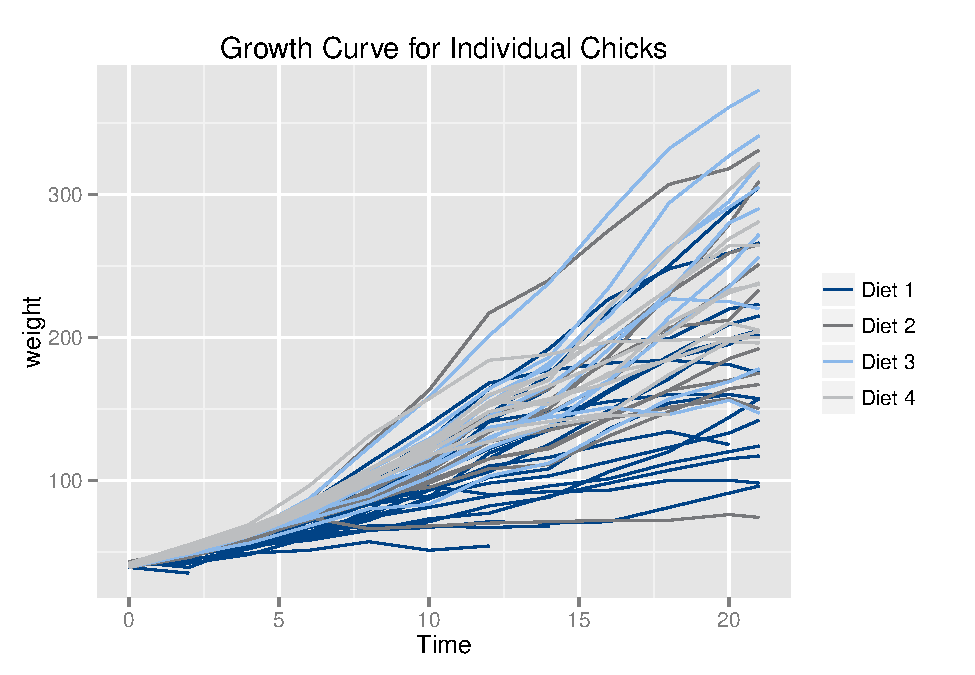
\includegraphics{Reproducible_Research_Demo_for_PLoS_files/figure-latex/unnamed-chunk-8-1} \end{CodeChunk}

Plot individual chick growth curves using small multiples.

\begin{CodeChunk}

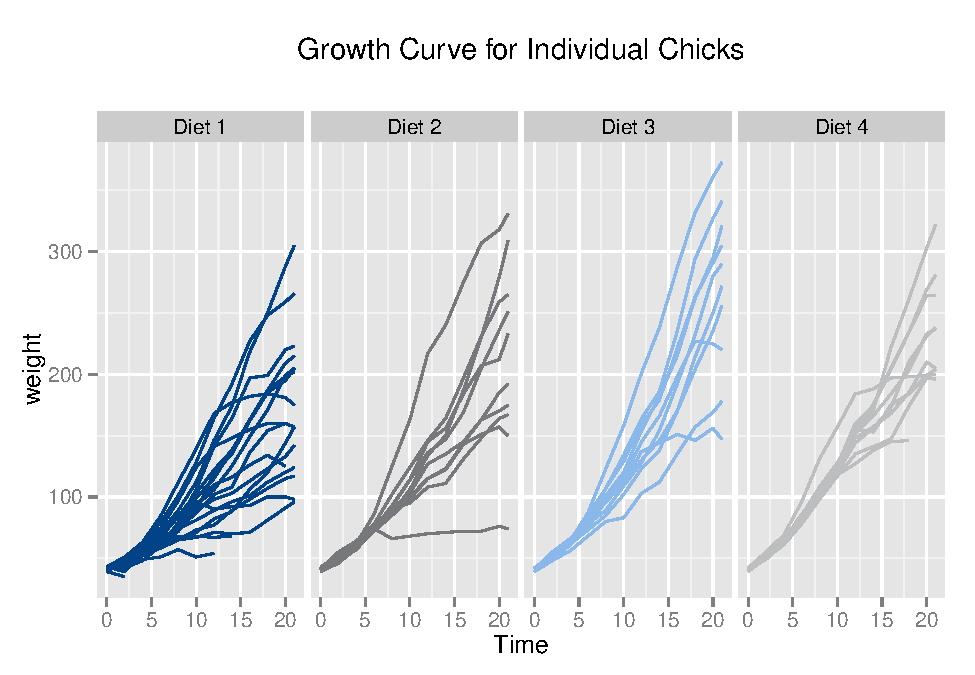
\includegraphics{Reproducible_Research_Demo_for_PLoS_files/figure-latex/unnamed-chunk-9-1} \end{CodeChunk}

Plot fitted growth curves using small multiples. Data points are
jittered around time value.

\begin{CodeChunk}

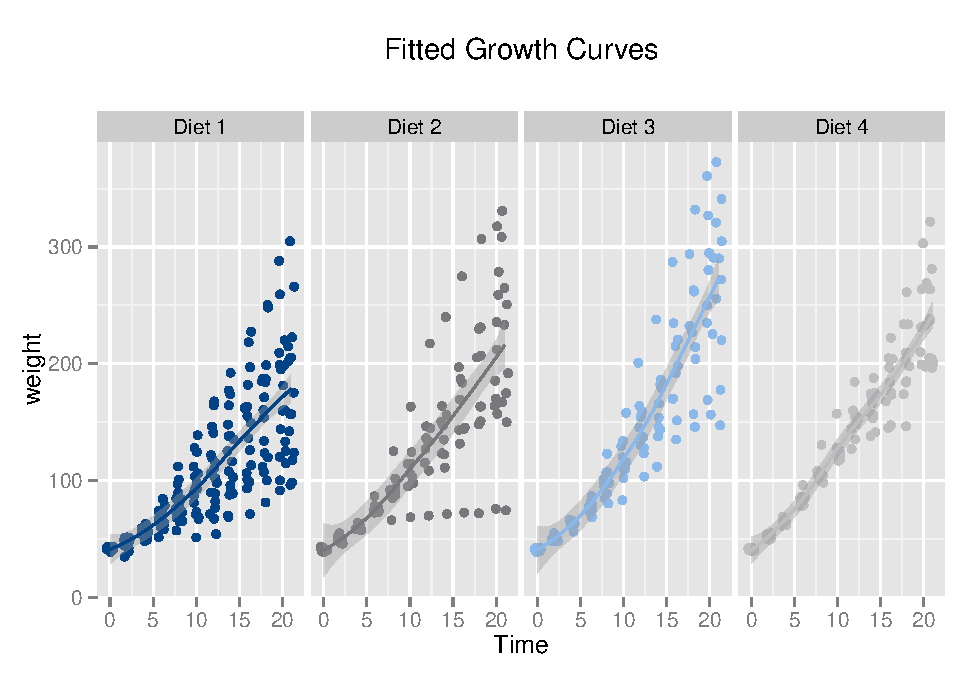
\includegraphics{Reproducible_Research_Demo_for_PLoS_files/figure-latex/unnamed-chunk-10-1} \end{CodeChunk}

\subsection*{Final weight density}\label{final-weight-density}
\addcontentsline{toc}{subsection}{Final weight density}

Plot densities by diet for chicks' final weights (day 21) using small
multiples.

\begin{CodeChunk}

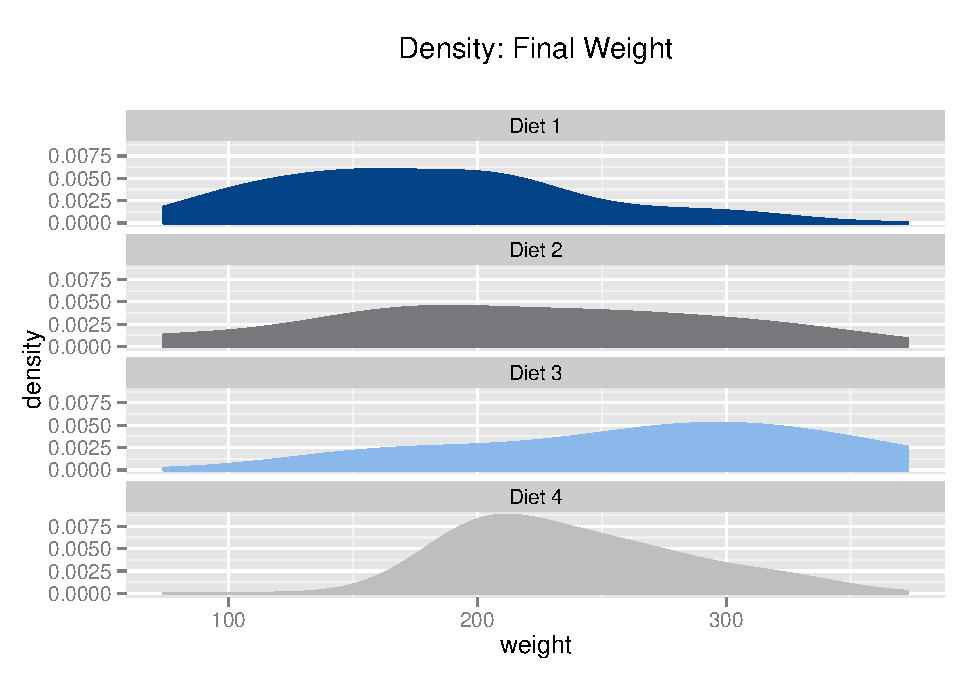
\includegraphics{Reproducible_Research_Demo_for_PLoS_files/figure-latex/unnamed-chunk-11-1} \end{CodeChunk}

\section*{Discussion}\label{discussion}
\addcontentsline{toc}{section}{Discussion}

Reproducibility rocks! End of discussion.

\section*{Material and Methods}\label{material-and-methods}
\addcontentsline{toc}{section}{Material and Methods}

Information on the R session that generated this paper is below.

\begin{CodeChunk}
\begin{CodeInput}
sessionInfo()
\end{CodeInput}
\begin{CodeOutput}
R version 3.1.3 (2015-03-09)
Platform: x86_64-w64-mingw32/x64 (64-bit)
Running under: Windows 7 x64 (build 7601) Service Pack 1

locale:
[1] LC_COLLATE=English_United States.1252 
[2] LC_CTYPE=English_United States.1252   
[3] LC_MONETARY=English_United States.1252
[4] LC_NUMERIC=C                          
[5] LC_TIME=English_United States.1252    

attached base packages:
[1] stats     graphics  grDevices utils     datasets  methods   base     

other attached packages:
[1] ggplot2_1.0.1    xtable_1.7-4     data.table_1.9.4

loaded via a namespace (and not attached):
 [1] chron_2.3-45     colorspace_1.2-6 digest_0.6.8     evaluate_0.7    
 [5] formatR_1.2      grid_3.1.3       gtable_0.1.2     htmltools_0.2.6 
 [9] knitr_1.10.5     labeling_0.3     magrittr_1.5     MASS_7.3-40     
[13] munsell_0.4.2    plyr_1.8.2       proto_0.3-10     Rcpp_0.11.6     
[17] reshape2_1.4.1   rmarkdown_0.6.1  rticles_1.0      scales_0.2.4    
[21] stringi_0.4-1    stringr_1.0.0    tools_3.1.3      yaml_2.1.13     
\end{CodeOutput}
\end{CodeChunk}

\section*{Acknowledgments}\label{acknowledgments}
\addcontentsline{toc}{section}{Acknowledgments}

Do NOT remove this, even if you are not including acknowledgments

\section*{References}\label{references}
\addcontentsline{toc}{section}{References}

A reference list should be automatically created here. However it won't.
Pandoc will place the list of references at the end of the document
instead. There are no convenient solution for now to force Pandoc to do
otherwise. The easiest way to get around this problem is to edit the
LaTeX file created by Pandoc before compiling it again using the
traditional LaTeX commands.

\section*{Figure Legends}\label{figure-legends}
\addcontentsline{toc}{section}{Figure Legends}

\section*{Tables}\label{tables}
\addcontentsline{toc}{section}{Tables}

1. Englander H, Michaels L, Chan B, Kansagara D (2014) The Care
Transitions Innovation (C-TraIn) for Socioeconomically Disadvantaged
Adults: Results of a Cluster Randomized Controlled Trial. J Gen Intern
Med.

2. Norris SL, McNally TK, Zhang X, Burda B, Chan B, et al. (2011)
Published norms underestimate the health-related quality of life among
persons with type 2 diabetes. J Clin Epidemiol 64: 358--365.

3. Melnikow J, Kulasingam S, Slee C, Helms LJ, Kuppermann M, et al.
(2010) Surveillance after treatment for cervical intraepithelial
neoplasia: outcomes, costs, and cost-effectiveness. Obstet Gynecol 116:
1158--1170.

4. Nelson HD, Tyne K, Naik A, Bougatsos C, Chan BK, et al. (2009)
Screening for breast cancer: an update for the U.S. Preventive Services
Task Force. Ann Intern Med 151: 727--737.

\end{document}

